\chapter{Track Simulation}
	In order to develop and test the~reconstruction algorithm, electron and positron tracks are simulated inside the~first detector sector $\mathcal{D}_1$ (see Section~\ref{sec:coor}) with different initial parameters (origin, initial direction and kinetic energy). Two approaches are currently used to simulate tracks, each of them for different purpose.
	
	The~\textbf{Microscopic Simulation} uses the~\garfieldpp toolkit~\cite{Garfield++}. Within this toolkit:
		\begin{enumerate}[nosep,label=\alph*)]
			\item \textcolor{red}{Magboltz, since it is mentioned later}
			\item the~\ac{HEED} program~\cite{HEED} is used to simulate the~primary particle,
			\item the~class \textit{AvalancheMicroscopic} to simulate the~drift of secondary electrons created by ionization in the~gas.
		\end{enumerate}
	This is the~most precise and time-consuming simulation used; our current goal is to be able to successfully reconstruct its results and determine our best-case energy resolution.
	
	The~\textbf{Runge-Kutta Simulation} uses the~4th order Runge-Kutta numerical integration (\textcolor{red}{add citation for Runge-Kutta}) to simulate the~trajectory of the~primary particle in the~electromagnetic field inside the~detector. It is relatively fast since it does not simulate the~secondary particles. It is used as part of our reconstruction algorithm and for testing some parts of the~reconstruction.
	
	All of these simulations require the~knowledge of the~electromagnetic field (both $\mathbf{E}$~and~$\mathbf{B}$) inside the~detector. A~uniform electric field of 400~V$\cdot$cm$^{-1}$ is assumed. The~magnetic field was simulated in Maxwell (see Section~\ref{sec:mag}). \textcolor{red}{add citation}
	
	\textcolor{red}{Single track in positive x direction or initial parameter randomization. Importance of gas composition, used gas compositions.}
	
	\section{Microscopic Simulation}
	\label{sec:microsim}
		The~microscopic simulation, the~most detailed simulation used in this work, is performed using the~\garfieldpp toolkit~\cite{Garfield++}.
		
		The~electron transport properties are simulated using the~program Magboltz~(\textcolor{red}{add citation,} \textcolor{orange}{details?}). Two different gas mixtures were compared -- 90:10 and 70:30 Ar:CO$_2$. The~second mixture will be used in our detector (\textcolor{orange}{this was probably known a~priori, but the first tests that I started with used 90/10, so maybe just note that the results justify the fact so far}). The~temperature is set to 20~$^\circ$C, the~pressure is atmospheric.
		
		The~primary track is simulated using the~program~\ac{HEED}, which is an implementation of the~photo-absorption ionization model~\cite{HEED} (\textcolor{orange}{see the reference, moved it to the end of sentence}). This program provides the~parameters of ionizing collisions. \ac{HEED} can also be used to simulate the~transport of delta electrons; we do not account for these in the~current simulation (\textcolor{orange}{but plan to include them in the~future -- maybe mention only in the conclusion/future section}). The~photons created in the~atomic relaxation cascade (\textcolor{red}{fluorescence reabsorption, ?}) are also not simulated.
		
		Finally, we use the~microscopic tracking provided by the~class \textit{AvalancheMicroscopic} in \garfieldpp to simulate the~drift of the~ionization electrons. Each electron is followed from collision to collision using the~equation of motion and the~collision rates calculated by Magboltz.
		
		\textcolor{red}{First simulated track in the~$z$ direction should be described in detail here (own subsection of the microscopic section, together with a~subsection for random/grid batches?). Figures.}
		
		\textcolor{red}{Add more detailed and better description of HEED, and microscopic tracking (each their own subsection?). Could also mention Monte Carlo (requires gas file generation - Magboltz) and Runge-Kutta simulation implemented in Garfield, why we don't use them (another subsection? rename the~section to \garfieldpp simulation and mention all relevant parts?).}
		
		\begin{figure}[H]
			\centering
			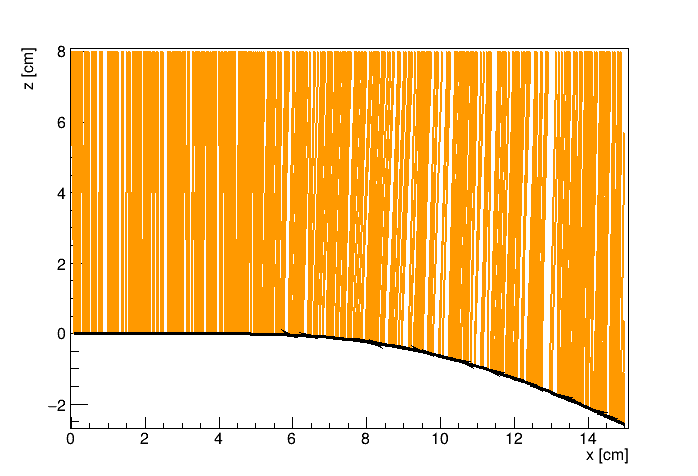
\includegraphics[width=0.3\textwidth]{7030_xz.png}
			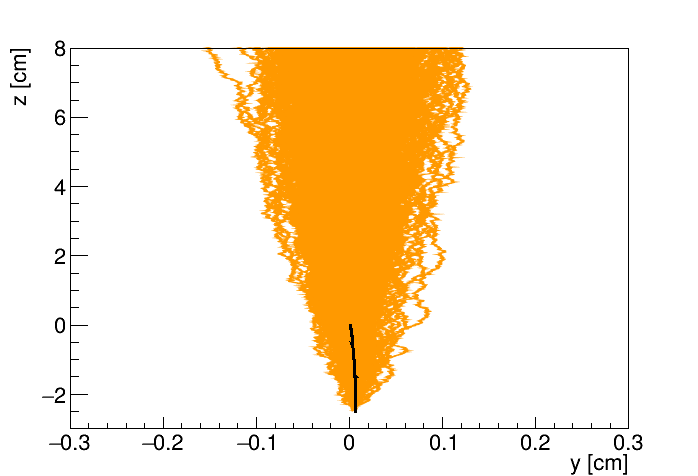
\includegraphics[width=0.3\textwidth]{7030_yz.png}
			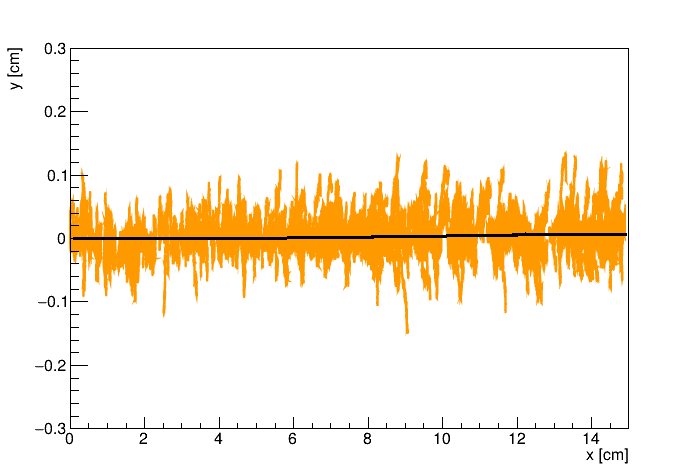
\includegraphics[width=0.3\textwidth]{7030_xy.png}
			\caption{Example of a~simulated electron track in 70~\%~argon and 30~\%~CO$_2$ atmosphere (on the~left). \textcolor{red}{Swap for better images, better zoom. Explain drift lines, primary particle.}}
			\label{fig:7030sim}
		\end{figure}
		
		\begin{figure}[H]
			\centering
			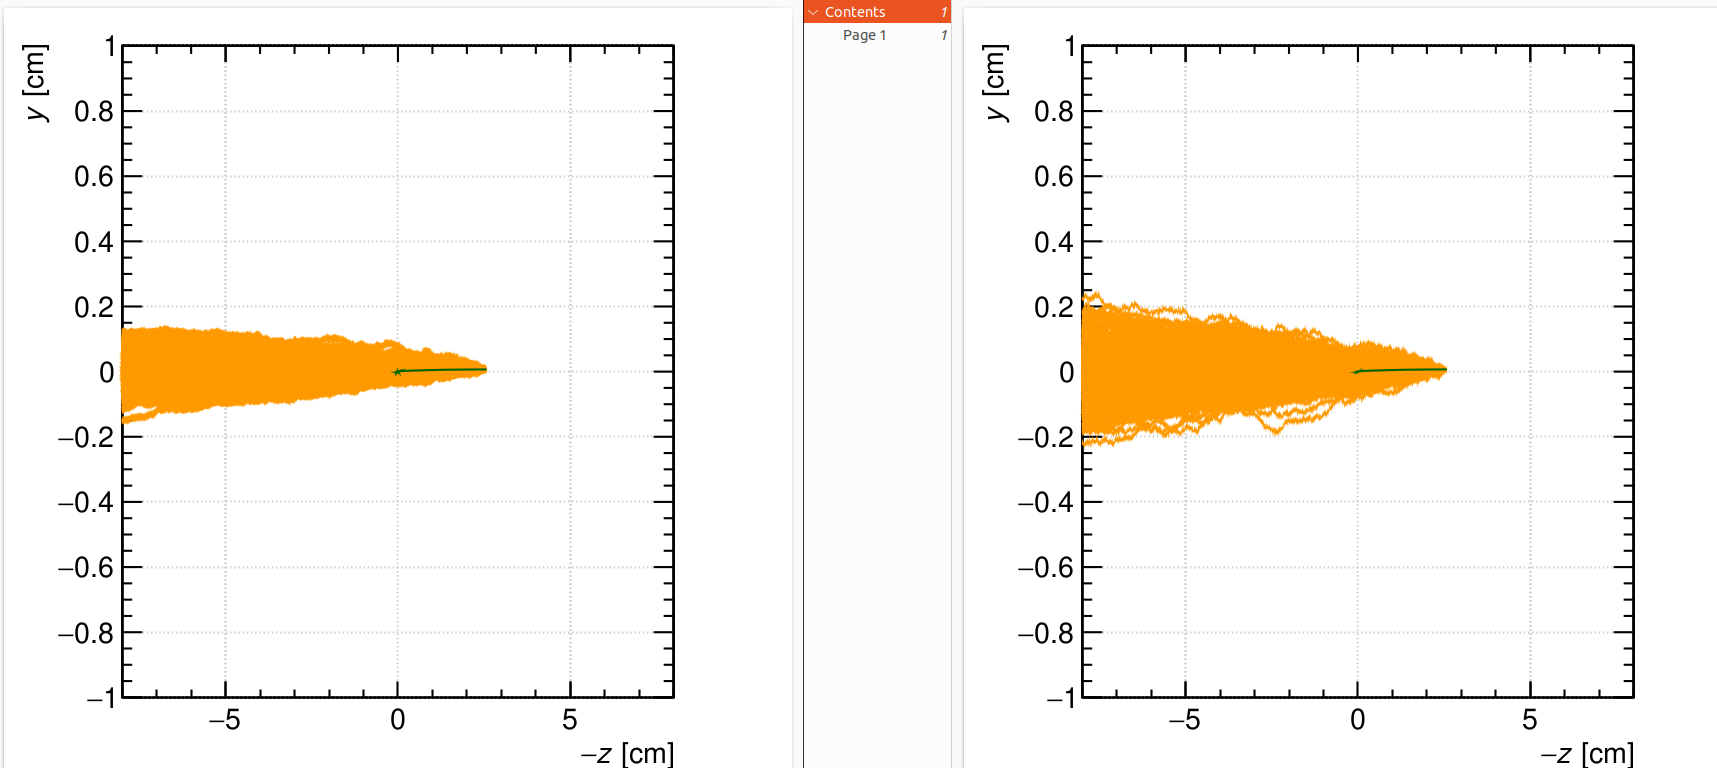
\includegraphics[width=0.9\textwidth]{diff_comp.png}
			\caption{Comparison of diffusion in a~simulated electron track in 70~\%~argon, 30~\%~CO$_2$ atmosphere and in 90~\%~argon, 10~\%~CO$_2$ atmosphere (on the~right). \textcolor{red}{Swap for better image, better zoom. Or put the~same pictures for both comparisons in one subfigure, etc. Describe better.}}
			\label{fig:diffcomp}
		\end{figure}
	
	\section{Runge-Kutta Simulation}
	\label{sec:rks}
		The~Runge-Kutta simulation in this work uses the~\ac{RK4} method to numerically integrate the~equation of motion of a~relativistic charged particle in an~electromagnetic field. Given a~system of first order differential equations
			\begin{equation}
				\derivative{\mathbf{y}}{t}(t) = \mathbf{f}(t,\mathbf{y}(t))
			\end{equation}
		with an initial condition
			\begin{equation}
				\mathbf{y}(t_0) = \mathbf{y}_0,
			\end{equation}
		we iteratively compute the estimate $\mathbf{y}_n = \mathbf{y}(t_n) = \mathbf{y}(t_0+nh)$ as follows (\textcolor{red}{citation? common knowledge?}):
			\begin{align}
				\mathbf{k}_1 &= \mathbf{f}(t_n,\mathbf{y}_n),\\
				\mathbf{k}_2 &= \mathbf{f}\left(t_n+\frac{h}{2},\, \mathbf{y}_n+\frac{h\mathbf{k}_1}{2}\right),\\
				\mathbf{k}_3 &= \mathbf{f}\left(t_n+\frac{h}{2},\, \mathbf{y}_n+\frac{h\mathbf{k}_2}{2}\right),\\
				\mathbf{k}_4 &= \mathbf{f}(t_n+h,\, \mathbf{y}_n+h\mathbf{k}_3),
			\end{align}
			\begin{equation}
				\mathbf{y}_{n+1} = \mathbf{y}_n + \frac{1}{6}(\mathbf{k}_1+2\mathbf{k}_2+2\mathbf{k}_3+\mathbf{k}_4).
			\end{equation}
		\textcolor{red}{Alternate forms (infinitely many) possible, accuracy vs computational cost. Runge-Kutta-Fehlberg with adaptive step size also possible, can potentially save some computation time especially in rapidly changing field (so maybe not in this case).}
		
		In our case, we want to integrate the~equation of motion, given by the~relativistic Lorentz force:
			\begin{equation}
				F^\mu_L = m\derivative{u^\mu}{\tau} = q F^{\mu\nu}u_{\nu},
			\end{equation}
		where the~Einstein summation convention is used, $m$~is the mass of the~particle, $q$~is its charge, $u^\mu$~is its four-velocity, $\tau$~is the~proper time (i.e., time in the~particle's frame of reference) and $F^{\mu\nu}$~is the~electromagnetic tensor at given coordinates~$x^\mu$ (we consider it to be time-independent in our detector). Given the electric $\mathbf{E} = (E_x,E_y,E_z)$ and the~magnetic field $\mathbf{B} = (B_x,B_y,B_z)$ and using the~metric signature $(+,-,-,-)$, the~equation expands to
			\begin{equation}
				\renewcommand{\arraystretch}{1.2}
				\derivative{}{\tau} \begin{pmatrix}\gamma c\\ \gamma v_x\\ \gamma v_y\\ \gamma v_z\end{pmatrix} = \frac{q}{m} 
				\begin{pmatrix}
					0             & -\frac{E_x}{c} & -\frac{E_y}{c} & -\frac{E_z}{c} \\
					\frac{E_x}{c} &  0             & -B_z           &  B_y           \\
					\frac{E_y}{c} &  B_z           &  0             & -B_x           \\
					\frac{E_z}{c} & -B_y           &  B_x           &  0
				\end{pmatrix}
				\begin{pmatrix}\gamma c\\ \gamma v_x\\ \gamma v_y\\ \gamma v_z\end{pmatrix},
				\renewcommand{\arraystretch}{1}
			\end{equation}
		where $c$ is the~speed of light in vacuum, $\mathbf{v} = (v_x,v_y,v_z)$ is the~particle's velocity and $\gamma = \left(1-\frac{v^2}{c^2}\right)^{-\frac{1}{2}}$ is the~Lorentz factor \textcolor{red}{(wrong magnetic field sign in the implementation???)}. Together with the~equation
			\begin{equation}
				\derivative{}{\tau} \begin{pmatrix} ct\\ x\\ y\\ z\end{pmatrix} = \begin{pmatrix}\gamma c\\ \gamma v_x\\ \gamma v_y\\ \gamma v_z\end{pmatrix} = u^\mu,
			\end{equation}
		we get a~system of eight first order differential equations for~$x^\mu$ and~$u^\mu$, which we can integrate using the~Runge-Kutta method described above. As a~result of this integration, we get the~position~$\mathbf{x}(\tau_n)$, the~velocity~$\mathbf{v}(\tau_n)$ and the~detector time~$t(\tau_n)$ for every proper time $\tau_n = n \tau_\text{step}$. \textcolor{red}{Integrating using the proper time means, that the step size in $t$ gets larger by the~gamma factor $\derivative{t}{\tau} = \gamma$ (maybe change it and integrate the~detector time or adjust the step size accordingly). The only difference is in the~step size (because $t$ gets also calculated as it is among the 8~variables)} As initial conditions, we use the~origin of the~track $(x_0,y_0,z_0)$, the~initial velocity direction vector $\mathbf{n} = (\cos\varphi\cos\theta,\sin\varphi\cos\theta,\sin\theta)$ and the~kinetic energy $E_\text{kin}$  (\textcolor{orange}{initial parameters of \textbf{the~simulation} (fit is in chapter 4)}), we then compute $\gamma$ and $\norm{\mathbf{v}}$:
			\begin{align}
				\gamma &= 1 + \frac{E_\text{kin}}{E_0},\\
				\norm{\mathbf{v}} &= c\sqrt{1-\gamma^{-2}}.
			\end{align}
		\textcolor{red}{Example of RK simulation -- first testing track, randomized sample of 100000 tracks.}